\documentclass[11pt]{article}

% ----------------------------------------------------------
% PACKAGES
% ----------------------------------------------------------
\usepackage[T1]{fontenc}
\usepackage[utf8]{inputenc}
\usepackage{lmodern}
\usepackage[margin=1in]{geometry}
\usepackage{amsmath, amssymb}
\usepackage{graphicx}
\usepackage{xcolor}
\usepackage{booktabs}
\usepackage{enumitem}
\usepackage{tikz}
\usepackage{framed}
\usepackage{setspace}
\usepackage{microtype}
\usepackage[hidelinks]{hyperref}
\usepackage[authoryear]{natbib}

% ----------------------------------------------------------
% CUSTOM MACROS (your notation commands)
% ----------------------------------------------------------
% ==========================================================
% EB-PAPERS: CANONICAL MACROS / COMMANDS
% Forecast Readiness Framework (FRF) / Electric Barometer
% ==========================================================
% Goals:
% - One meaning per symbol.
% - Shared across all papers/notes/briefs.
% - Backwards-compatible aliases.
% - Avoid redefinition errors via \providecommand.
% ==========================================================

% ----------------------------------------------------------
% Core framework / artifacts
% ----------------------------------------------------------
\providecommand{\FRF}{\ensuremath{\mathrm{FRF}}}
\providecommand{\FRS}{\ensuremath{\mathrm{FRS}}}

\providecommand{\FPC}{\ensuremath{\mathrm{FPC}}}
\providecommand{\DQC}{\ensuremath{\mathrm{DQC}}}
\providecommand{\Governance}{\ensuremath{\mathrm{Governance}}}
\providecommand{\GovernanceDecision}{\ensuremath{\mathrm{GovernanceDecision}}}

\providecommand{\RAL}{\ensuremath{\mathrm{RAL}}}

% Readiness primitives / governance vocabulary
\providecommand{\ReadinessPrimitive}{\ensuremath{\mathrm{RP}}}

% Limited-Time Offers
\providecommand{\LTO}{\ensuremath{\mathrm{LTO}}}
\providecommand{\LTOs}{\ensuremath{\mathrm{LTOs}}}

% ----------------------------------------------------------
% Core metrics (upright math)
% ----------------------------------------------------------
\providecommand{\CWSL}{\ensuremath{\mathrm{CWSL}}}
\providecommand{\CWSLR}{\ensuremath{\mathrm{CWSLR}}} % named artifact in prose
\providecommand{\NSL}{\ensuremath{\mathrm{NSL}}}
\providecommand{\UD}{\ensuremath{\mathrm{UD}}}
\providecommand{\HR}{\ensuremath{\mathrm{HR}}}
\providecommand{\HRtau}{\ensuremath{\mathrm{HR}@\tau}}

% FRS sub-terms
\providecommand{\CWSLscaled}{\ensuremath{\mathrm{CWSL}_{\mathrm{scaled}}}}
\providecommand{\CWSLmax}{\ensuremath{\mathrm{CWSL}_{\max}}}

% Legacy HR macro names
\providecommand{\HRAT}{\ensuremath{\mathrm{HR@\tau}}}
\providecommand{\tauTol}{\ensuremath{\tau}}
\providecommand{\tauop}{\ensuremath{\tau}}

% ----------------------------------------------------------
% Indexing and sets
% ----------------------------------------------------------
\providecommand{\Iset}{\ensuremath{I}}
\providecommand{\Tset}{\ensuremath{T}}

\providecommand{\entity}{\ensuremath{i}}
\providecommand{\timeindex}{\ensuremath{t}}

% Back-compat index shorthands
\providecommand{\iidx}{\entity}
\providecommand{\tidx}{\timeindex}

% Summation shorthand
\providecommand{\sumit}{\ensuremath{\sum_{\entity \in \Iset} \sum_{\timeindex \in \Tset}}}

% Optional sizes / counts
\providecommand{\Tsize}{\ensuremath{|\Tset|}}
\providecommand{\nobs}{\ensuremath{N}}

% ----------------------------------------------------------
% Forecast / demand notation
% ----------------------------------------------------------
\providecommand{\y}{\ensuremath{y}}
\providecommand{\yhat}{\ensuremath{\hat{y}}}

\providecommand{\yit}{\ensuremath{y_{\entity\timeindex}}}
\providecommand{\yhatit}{\ensuremath{\hat{y}_{\entity\timeindex}}}

% Common residuals / errors
\providecommand{\errit}{\ensuremath{e_{\entity\timeindex}}}
\providecommand{\resit}{\errit} % alias
\providecommand{\absit}{\ensuremath{\left|\yhatit - \yit\right|}}
\providecommand{\abserrit}{\absit} % alias

% Explicit residual definition macro (optional)
\providecommand{\resdef}{\ensuremath{\errit = \yit - \yhatit}}

% ----------------------------------------------------------
% Shortfall / overbuild decomposition
% ----------------------------------------------------------
\providecommand{\shortfall}{\ensuremath{s}}
\providecommand{\overbuild}{\ensuremath{o}}

\providecommand{\sit}{\ensuremath{s_{\entity\timeindex}}}
\providecommand{\oit}{\ensuremath{o_{\entity\timeindex}}}

% Positive-part operator (canonical name)
\providecommand{\pospart}[1]{\left(#1\right)_{+}}

% Explicit decompositions
\providecommand{\shortfalldef}{\ensuremath{\sit = \pospart{\yit - \yhatit}}}
\providecommand{\overbuilddef}{\ensuremath{\oit = \pospart{\yhatit - \yit}}}

% Back-compat convenience symbols used in some notes
\providecommand{\sdepth}{\shortfall} % UD paper convenience

% ----------------------------------------------------------
% Indicators / expectations / operators
% ----------------------------------------------------------
% Canonical indicator: \Ind{event}
\providecommand{\Ind}{\ensuremath{\mathbb{I}}}
\providecommand{\indicator}[1]{\ensuremath{\mathbf{1}\{#1\}}} % prose-friendly alternative

% Back-compat: some notes used \Indicator (capital I). Keep as an alias to the
% canonical \Ind to avoid duplicate meanings.
\providecommand{\Indicator}{\Ind}

% If you want function-style indicator without braces: \Ind\!(event)
% Keep as \Ind and let authors decide.
\providecommand{\E}{\ensuremath{\mathbb{E}}}

\providecommand{\abs}[1]{\left|#1\right|}
\providecommand{\card}[1]{\left|#1\right|}

% ----------------------------------------------------------
% Cost parameters + cost ratio calibration (CWSLR note)
% ----------------------------------------------------------
% IMPORTANT: Canonical costs are subscripted (c_u, c_o). This avoids
% collisions with superscript variants.
\providecommand{\cu}{\ensuremath{c_u}}
\providecommand{\co}{\ensuremath{c_o}}

% Entity-specific costs
\providecommand{\cui}{\ensuremath{c_{u,\entity}}}
\providecommand{\coi}{\ensuremath{c_{o,\entity}}}

% Cost ratio
\providecommand{\R}{\ensuremath{R}}
\providecommand{\Ri}{\ensuremath{R_{\entity}}}
\providecommand{\Rdef}{\ensuremath{R = \cu/\co}}

% Aggregate under/over cost functions (used in calibration prose)
\providecommand{\UnderCost}{\ensuremath{\mathrm{UnderCost}}}
\providecommand{\OverCost}{\ensuremath{\mathrm{OverCost}}}

% Candidate grid
\providecommand{\Rgrid}{\ensuremath{\mathcal{R}}}

% Calibrated selections
\providecommand{\Rstar}{\ensuremath{R^{\ast}}}
\providecommand{\Rist}{\ensuremath{R^{\ast}_{\entity}}}

% CWSL as a function of R (notation)
\providecommand{\CWSLofR}{\ensuremath{\CWSL(\R)}}
\providecommand{\CWSLofRi}{\ensuremath{\CWSL(\Ri)}}

% Balance-based selection operator (kept as a macro because you used it)
\providecommand{\Rbalance}{%
\ensuremath{%
\arg\min_{\R \in \Rgrid}\left|\UnderCost(\R) - \OverCost(\R)\right|%
}%
}

% Back-compat (older notes used superscripts c^u / c^o)
\providecommand{\cuSup}{\ensuremath{c^{u}}}
\providecommand{\coSup}{\ensuremath{c^{o}}}
\providecommand{\cuiSup}{\ensuremath{c^{u}_{\entity}}}
\providecommand{\coiSup}{\ensuremath{c^{o}_{\entity}}}

% ----------------------------------------------------------
% HR@tau scanning / calibration (HRtau note)
% ----------------------------------------------------------
\providecommand{\tauval}{\ensuremath{\tau}}
\providecommand{\tauv}{\tauval}
\providecommand{\taui}{\ensuremath{\tau_{\entity}}}

% Candidate tolerance grid
\providecommand{\TauGrid}{\ensuremath{\mathcal{T}}}

% Calibrated tolerances
\providecommand{\taustar}{\ensuremath{\tau^{\ast}}}
\providecommand{\taustari}{\ensuremath{\tau^{\ast}_{\entity}}}

% Target hit-rate (if used)
\providecommand{\hstar}{\ensuremath{h^{\ast}}}

% Hit indicator definition helpers
\providecommand{\Hitit}{\ensuremath{h_{\entity\timeindex}}}
\providecommand{\HitDef}{\ensuremath{\Hitit = \Ind\!\left(\absit \le \tauval\right)}}

% HR as a function of tau
\providecommand{\HRoftau}{\ensuremath{\HR(\tauval)}}
\providecommand{\HRtauoftau}{\ensuremath{\HRtau(\tauval)}}

% Optional utility selection helpers
\providecommand{\lambdau}{\ensuremath{\lambda}}
\providecommand{\taumax}{\ensuremath{\tau_{\max}}}
\providecommand{\Utility}{\ensuremath{\mathcal{U}}}
\providecommand{\UtilityDef}{\ensuremath{\Utility(\tauval) = \HR(\tauval) - \lambdau \cdot (\tauval/\taumax)}}

% Governance guards
\providecommand{\taufloor}{\ensuremath{\tau_{\min}}}
\providecommand{\taucap}{\ensuremath{\tau_{\mathrm{cap}}}}
\providecommand{\nmin}{\ensuremath{n_{\min}}}

% ----------------------------------------------------------
% DQC / snapping / quantization (DQC note)
% ----------------------------------------------------------
\providecommand{\gunit}{\ensuremath{g}}
\providecommand{\guniti}{\ensuremath{g_{\entity}}}

\providecommand{\ygrid}{\ensuremath{\tilde{y}}}
\providecommand{\ygridit}{\ensuremath{\tilde{y}_{\entity\timeindex}}}

\providecommand{\yhatgrid}{\ensuremath{\tilde{\hat{y}}}}
\providecommand{\yhatgridit}{\ensuremath{\tilde{\hat{y}}_{\entity\timeindex}}}

\providecommand{\snap}{\ensuremath{\mathcal{S}}}
\providecommand{\snaphatdef}{\ensuremath{\yhatgridit = \snap_{\gunit}\!\left(\yhatit\right)}}
\providecommand{\snapydef}{\ensuremath{\ygridit = \snap_{\gunit}\!\left(\yit\right)}}

\providecommand{\residit}{\ensuremath{r_{\entity\timeindex}}}
\providecommand{\residdef}{\ensuremath{\residit = \yit - \ygridit}}

\providecommand{\MAD}{\ensuremath{\mathrm{MAD}}}
\providecommand{\IQR}{\ensuremath{\mathrm{IQR}}}

\providecommand{\multirate}{\ensuremath{\rho}}
\providecommand{\multiratei}{\ensuremath{\rho_{\entity}}}

\providecommand{\DeltaStar}{\ensuremath{\Delta^{\ast}}}

\providecommand{\Pset}{\ensuremath{\mathcal{P}}}
\providecommand{\packunit}{\ensuremath{p}}
\providecommand{\packuniti}{\ensuremath{p_{\entity}}}

% DQC classes
\providecommand{\ContinuousLike}{\textsc{Continuous-like}}
\providecommand{\Quantized}{\textsc{Quantized}}
\providecommand{\PiecewisePacked}{\textsc{Piecewise-packed}}

% FPC classes
\providecommand{\Compatible}{\textsc{Compatible}}
\providecommand{\Marginal}{\textsc{Marginal}}
\providecommand{\Incompatible}{\textsc{Incompatible}}

% ----------------------------------------------------------
% RAL shorthands used in notes
% ----------------------------------------------------------
\providecommand{\alphaadj}{\ensuremath{\alpha}}

% RAL operator (functional form)
\providecommand{\RALop}{\ensuremath{\mathcal{R}_{\alphaadj}}}

\providecommand{\yhatadjit}{\ensuremath{\hat{y}^{(\alphaadj)}_{\entity\timeindex}}}
\providecommand{\yhatadjdef}{\ensuremath{\yhatadjit = (1+\alphaadj)\,\yhatit}}

\providecommand{\dNSL}{\ensuremath{\Delta \NSL}}
\providecommand{\dHRtau}{\ensuremath{\Delta \HRtau}}
\providecommand{\dCWSL}{\ensuremath{\Delta \CWSL}}

% ----------------------------------------------------------
% Governance policy handles
% ----------------------------------------------------------
\providecommand{\TauPolicy}{\ensuremath{\mathrm{TauPolicy}}}
\providecommand{\RALPolicy}{\ensuremath{\mathrm{RALPolicy}}}
\providecommand{\UnitPolicy}{\ensuremath{\mathrm{UnitPolicy}}}

\providecommand{\GovernanceStatus}{\ensuremath{\mathrm{GovernanceStatus}}}
\providecommand{\Green}{\textsc{Green}}
\providecommand{\Yellow}{\textsc{Yellow}}
\providecommand{\Red}{\textsc{Red}}

\providecommand{\RawUnits}{\textsc{Raw}}
\providecommand{\SnappedUnits}{\textsc{Snapped}}

% ----------------------------------------------------------
% LTO paper specifics
% ----------------------------------------------------------
\providecommand{\ltoOn}{\ensuremath{z_{\timeindex}}}
\providecommand{\ltoPhase}{\ensuremath{\phi_{\timeindex}}}
\providecommand{\qprod}{\ensuremath{\mathrm{QP}}}

% ----------------------------------------------------------
% Frontmatter helpers
% ----------------------------------------------------------
\providecommand{\keywords}[1]{%
\par\noindent\textbf{Keywords: }#1\par
}

% ----------------------------------------------------------
% Prose shorthands
% ----------------------------------------------------------
\providecommand{\ie}{i.e.\ }
\providecommand{\eg}{e.g.\ }

% ==========================================================
% END
% ==========================================================


% ----------------------------------------------------------
% PDF METADATA
% ----------------------------------------------------------
\hypersetup{
    pdftitle={Cost-Weighted Service Loss: A Forecast Evaluation Metric for Operational Readiness Under Asymmetric Error Cost},
    pdfauthor={Kyle Corrie},
    colorlinks=true,
    linkcolor=blue,
    citecolor=blue,
    urlcolor=blue
}

% ----------------------------------------------------------
% TITLE PAGE
% ----------------------------------------------------------
\title{
\textbf{Cost-Weighted Service Loss (CWSL):}\\[4pt]
{\large A Forecast Evaluation Metric Aligned with Operational Asymmetry}
}

\author{
  Kyle Corrie\\[4pt]
  \small Electric Barometer Series\\
  \small \texttt{kcorrie@economistician.com}
}

\date{December 2025\\[4pt]\small Working Paper --- Electric Barometer Series\\Version 0.1}

% ==================================================
\begin{document}

\maketitle

% ----------------------------------------------------------
% ORDERED SECTION INPUTS
% ----------------------------------------------------------
% ==========================================================
% 000_frontmatter.tex
% FRONTMATTER (Forecast Governance Technical Note)
% ==========================================================

\begin{abstract}
Operational forecasting systems increasingly embed evaluation diagnostics directly
into downstream decisions, policy gates, and automated readiness interventions.
In such settings, it is not sufficient to compute cost-aware error or service
metrics. One must also establish that both the \emph{units of interpretation} and
the \emph{forecast primitive itself} are structurally admissible for the observed
demand process.

This technical note introduces \emph{Forecast Governance} as a deterministic,
auditable decision contract that composes two companion diagnostics:
\emph{Demand Quantization Compatibility (DQC)}, which determines whether evaluation
and control must respect a discrete demand representation, and
\emph{Forecast Primitive Compatibility (FPC)}, which determines whether readiness
adjustment constitutes a valid control lever under that representation.

Governance produces a single authoritative artifact—the
\texttt{GovernanceDecision}—that specifies representation requirements, tolerance
semantics, readiness allowability, and compliance status with explicit rationale.
Forecast Governance is not a performance metric and is not an optimization
objective. It is a policy layer designed to ensure that evaluation semantics are
well-defined before downstream optimization, selection, or control is attempted.
\end{abstract}

% ----------------------------------------------------------
% INTRODUCTION
% ----------------------------------------------------------
\section{Introduction}

Forecasts play a central role in operational decision-making in environments where
timing, readiness, and service reliability matter. Quick-service restaurants (QSR),
retail stores, production lines, and high-frequency inventory systems all rely on
forecasts to ensure that product, labor, or capacity is available exactly when needed.
In such environments, forecast errors translate directly into operational outcomes.

Most organizations evaluate forecast performance using symmetric accuracy metrics such
as mean absolute error (MAE), root mean squared error (RMSE), and mean absolute
percentage error (MAPE). These measures treat equal-magnitude errors identically
regardless of direction, implicitly assuming that the operational cost of
under-forecasting is no different from the cost of over-forecasting. However, this
assumption rarely holds in practice. Under-forecasting often produces service failures,
unmet demand, and elevated operational stress, while over-forecasting typically leads
to excess production or inventory that carries far lower cost.

This mismatch between statistical evaluation and operational impact can lead
organizations to select models that appear accurate on paper yet consistently produce
readiness failures. Forecasts may achieve low MAPE while still causing shortfalls during
peak periods—precisely when operational reliability is most important. As organizations
increasingly rely on short-horizon forecasts for high-frequency decisions, symmetric
evaluation metrics become inadequate for assessing real operational performance.

To address this gap, this paper introduces the \textit{Cost-Weighted Service Loss
(CWSL)} metric, which evaluates forecast performance by explicitly incorporating
asymmetric penalties for shortfalls and overbuilds and normalizing results by total
demand. CWSL is complemented by supporting measures that provide insight into
reliability, tolerance accuracy, and the severity of shortfalls. Together, these metrics
offer a practical and interpretable framework for assessing forecast quality in
environments where direction, magnitude, and operational consequence all matter.
% ----------------------------------------------------------
% RELATED WORK
% ----------------------------------------------------------
\section{Related Work}

Forecast accuracy is traditionally assessed using symmetric error metrics such as mean
absolute error (MAE), root mean squared error (RMSE), and mean absolute percentage error
(MAPE). These metrics are widely adopted due to their simplicity, interpretability, and
compatibility with diverse modeling approaches \cite{hyndman2018}. However, they treat
forecast deviations symmetrically and thus implicitly assume that over-forecasting and
under-forecasting impose equivalent cost. In settings where shortages are substantially
more disruptive than excess, this assumption leads to evaluations that obscure the
operational consequences most relevant to managers \cite{goodwin2011}.

A long-standing literature in operations management emphasizes the asymmetric cost of
shortages and excess. The classic newsvendor formulation \cite{arrow1951} captures
underage and overage cost asymmetry and shows that optimal inventory decisions depend on
their relative magnitudes. Subsequent research extends these ideas to service-level
constraints, multi-echelon systems, perishability, and risk preferences. However, these
models are designed for \textit{decision optimization} rather than \textit{forecast
evaluation}, and typically do not characterize interval-level forecast error or provide
metrics for assessing forecast quality.

Asymmetric loss functions also appear in statistical and machine learning contexts.
Quantile (pinball) loss \cite{koenker2005} penalizes over-prediction and
under-prediction unequally, and is widely used for distributional forecasting and
predictive uncertainty estimation. Other work has explored tilted or cost-weighted loss
functions in classification and regression to encode domain-specific risk preferences
\cite{gneiting2011}. While related in spirit, these methods influence \textit{model
training} rather than evaluation of realized forecast output, and they do not normalize
costs by demand or incorporate operational readiness concepts.

Forecast evaluation specifically in operational environments has received increased
attention across domains such as retail replenishment \cite{ferreira2016}, call center
management \cite{audi2019}, workforce scheduling \cite{gans2003}, and intermittent
demand forecasting \cite{snyder2012}. These studies highlight the importance of aligning
forecasts with service levels, staffing requirements, or production constraints.
Nevertheless, existing evaluation approaches are primarily symmetric or rely on
volume-normalized measures such as wMAPE, which cannot differentiate between error
patterns that are operationally benign and those that produce readiness failures.

Across these literatures, we are not aware of an evaluation framework that jointly
integrates:
(1) explicit asymmetric penalties for shortfalls and overbuilds;
(2) demand normalization across items and intervals; and
(3) interval-level granularity suitable for high-frequency operational environments.

The Cost-Weighted Service Loss (CWSL) metric introduced in this paper fills this gap by
adapting asymmetric cost principles into a forecast evaluation framework that is both
operationally interpretable and widely applicable across domains where readiness and
service reliability are central performance objectives.
% ----------------------------------------------------------
% CONTRIBUTIONS
% ----------------------------------------------------------
\section{Contributions}

This paper makes three primary contributions to the forecasting and operations
management literature:

\begin{enumerate}[itemsep=8pt]
    \item \textbf{A new forecast evaluation metric grounded in asymmetric operational
    cost.} We introduce \textit{Cost-Weighted Service Loss (CWSL)}, a demand-normalized
    metric that incorporates explicit penalties for shortfalls and overbuilds. CWSL
    captures the directional consequences of forecast error at the interval level,
    addressing a gap in existing evaluation methods that assume symmetric cost.

    \item \textbf{A diagnostic framework for operational readiness assessment.} Beyond the primary metric, we develop four complementary measures—No-Shortfall Level (NSL), Hit Rate within Tolerance (HR@\(\tau\)), Underbuild Depth (UD), and the Forecast Readiness Score (FRS). Together, these metrics provide a structured approach for identifying failure modes, assessing tolerance accuracy, and quantifying the severity of operational shortfalls, and they are defined in a way that supports aggregation across items, categories, stores, and other operational hierarchies.

    \item \textbf{Evidence of cross-domain applicability and operational relevance.}
    Through illustrative examples and industry-specific discussion, we demonstrate how
    CWSL applies to a wide range of high-frequency operational settings, including QSR,
    retail replenishment, manufacturing, logistics, workforce planning, and energy load
    forecasting. This highlights the generalizability of CWSL as a unifying framework for
    evaluating forecast performance under asymmetric error structures.
\end{enumerate}

These contributions position CWSL as both a methodological advancement and a practical
tool for organizations seeking to align forecasting evaluation with operational
priorities.
% ----------------------------------------------------------
% OPERATIONAL MOTIVATION
% ----------------------------------------------------------
\section{Operational Motivation}

The consequences of forecast error depend not only on magnitude but on direction. In
many operational environments, under-forecasting creates service disruptions: unmet
demand, slower throughput, operational recovery time, and even reputational risk.
Over-forecasting, by contrast, typically results in manageable waste or slight
inefficiencies. This directional asymmetry forms the foundation for cost-weighted
evaluation.

% 040_asymmetry_cost_curve.tex
% Conceptual illustration of asymmetric cost penalties

\begin{figure}[h!]
\centering
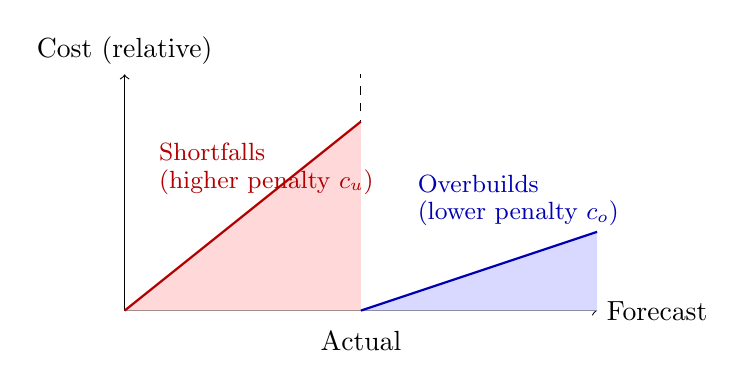
\begin{tikzpicture}[scale=1]

  % Axes
  \draw[->] (0,0) -- (6,0) node[right] {Forecast};
  \draw[->] (0,0) -- (0,3) node[above] {Cost (relative)};

  % Vertical line at Actual
  \draw[dashed] (3,0) -- (3,3);
  \node[below=4pt] at (3,0) {Actual};

  % Shortfall region
  \fill[red!15] (0,0) -- (3,0) -- (3,2.4) -- cycle;
  \draw[red!70!black, thick] (0,0) -- (3,2.4);
  \node[red!70!black, align=left] at (1.8,1.8)
      {\small Shortfalls\\[-2pt]\small (higher penalty $c_u$)};

  % Overbuild region
  \fill[blue!15] (3,0) -- (6,0) -- (6,1.0) -- cycle;
  \draw[blue!70!black, thick] (3,0) -- (6,1.0);
  \node[blue!70!black, align=left] at (5.0,1.4)
      {\small Overbuilds\\[-2pt]\small (lower penalty $c_o$)};

\end{tikzpicture}
\caption{Conceptual illustration of asymmetric penalties: shortfalls incur a higher
penalty ($c_u$) than overbuilds ($c_o$).}
\label{fig:asymmetry}
\end{figure}

Shortfalls may cause lost transactions, slower service, or staffing reallocations.
Overbuilds rarely require recovery; they simply incur modest excess. Across items,
dayparts, and locations, this asymmetry varies but is consistently present.
% ----------------------------------------------------------
% CWSL METHODOLOGY
% ----------------------------------------------------------
\section{Methodology: Cost-Weighted Service Loss (CWSL)}

This section formalizes the Cost-Weighted Service Loss (CWSL) metric and its supporting
diagnostic measures. Our objective is to construct a forecast evaluation framework that
reflects the asymmetric operational consequences of under-forecasting and
over-forecasting, while remaining interpretable, demand-normalized, and applicable
across items and intervals. We begin by defining shortfall and overbuild components,
introduce asymmetric penalty weights, and present the formal CWSL definition. We then
describe supplementary metrics designed to quantify service reliability, tolerance
accuracy, and shortfall severity.

\subsection{Shortfall and Overbuild Components}

Let \(\mathcal{I}\) denote the set of items (or commodities) and \(\mathcal{T}\) the set
of evaluation intervals. For item \(i \in \mathcal{I}\) and interval \(t \in \mathcal{T}\),
let \(y_{it}\) denote the actual demand and \(\hat{y}_{it}\) the corresponding forecast.
Forecast error can be decomposed into two nonnegative components:
\[
s_{it} = \max(0,\, y_{it} - \hat{y}_{it}) \qquad \text{(shortfall)},
\]
\[
o_{it} = \max(0,\, \hat{y}_{it} - y_{it}) \qquad \text{(overbuild)}.
\]

This decomposition ensures that only one component is positive for any \((i,t)\) pair.
Shortfalls capture instances where demand exceeds the forecast, while overbuilds capture
instances where production or allocation exceeded realized demand. This
directionally-aware formulation is essential in environments where operational cost is
not symmetric around zero error.

\subsection{Asymmetric Penalty Weights}

The shortfall and overbuild components \(s_{it}\) and \(o_{it}\) become operationally
meaningful once they are linked to the relative cost of being short versus long.
Operational evidence consistently demonstrates that the cost of under-forecasting
short-horizon demand exceeds the cost of over-forecasting. Shortfalls may lead to unmet
demand, slower service, inventory depletion, or labor reallocation. Overbuilds, by
contrast, typically incur modest waste or holding cost. To reflect this asymmetry, we
assign each item \(i\) two nonnegative penalty parameters:

\begin{itemize}[itemsep=4pt]
    \item \(c_{u,i}\): unit penalty for shortfalls,
    \item \(c_{o,i}\): unit penalty for overbuilds, typically \(c_{u,i} > c_{o,i}\).
\end{itemize}

These penalties may differ across items due to recovery times, perishability, guest
impact, or cost of waste. In the baseline formulation, we treat \(c_{u,i}\) and
\(c_{o,i}\) as fixed for each item over the evaluation horizon, but the framework
readily extends to time- or context-varying penalties (e.g., by daypart or service
window). CWSL therefore permits full item-level flexibility, allowing penalties to
reflect operational realities rather than assuming uniform cost across the product mix.

Throughout this paper, we refer to \(c_{u,i} s_{it} + c_{o,i} o_{it}\) as a
\emph{cost-weighted penalty}. These penalty weights need not correspond to literal
currency values; rather, they encode the \emph{relative} operational impact of
shortfalls and overbuilds for each item. This distinction allows CWSL to remain flexible
across domains while still capturing the directional asymmetry inherent in operational
cost.

\subsection{Selecting Cost Parameters}

The penalty parameters \(c_{u,i}\) and \(c_{o,i}\) encode an organization’s view of the
relative cost of shortfalls and overbuilds for item \(i\). In principle, these
quantities could be expressed in monetary terms (e.g., lost margin versus waste cost),
but in many operational settings it is sufficient---and often more practical---to work
with \emph{relative} penalties that summarize how much worse it is to be short than to
be long. In this subsection we outline simple, practitioner-oriented guidance for
selecting cost parameters that is consistent with the CWSL framework and scalable across
items.

\subsubsection*{Operational Judgment (Practical Baseline)}

In organizations without detailed cost accounting or where the drivers of shortfall cost
are diffuse (e.g., lost throughput, guest dissatisfaction, recovery time), it is rarely
feasible to pin down exact currency-valued penalties for every item. In such cases,
CWSL can be parameterized using structured managerial judgment.

A natural starting point is to work with the \emph{penalty ratio}
\[
R_i = \frac{c_{u,i}}{c_{o,i}},
\]
which summarizes how many times more costly a unit of shortfall is than a unit of
overbuild for item \(i\). Rather than specifying \(c_{u,i}\) and \(c_{o,i}\) separately,
practitioners can first elicit an approximate value of \(R_i\) and then choose
convenient scaled penalties (e.g., \(c_{o,i} = 1\), \(c_{u,i} = R_i\)).

In practice, this can be implemented through structured discussions with operations
leaders, store managers, or production supervisors. For each item (or item group),
managers can be asked qualitative questions such as:
\begin{itemize}[itemsep=4pt]
    \item ``If we are short by one unit in a peak interval, is that roughly two times,
          five times, or ten times worse than having one unit left over?''
    \item ``For this item, would you rather be slightly long most of the time, or risk
          being short in exchange for lower waste?''
\end{itemize}
Their responses can be mapped to simple, interpretable ratios, for example:
\begin{itemize}[itemsep=4pt]
    \item \emph{Moderately asymmetric} environments: \(R_i \in [2,4]\),
    \item \emph{Strongly asymmetric} environments (e.g., core items during peaks):
          \(R_i \in [5,8]\),
    \item \emph{Extremely asymmetric} environments (e.g., critical bottleneck items):
          \(R_i \ge 8\).
\end{itemize}

Once an approximate ratio has been selected, penalties can be normalized without loss of
generality. A common convention is to set \(c_{o,i} = 1\) for all items and let
\(c_{u,i} = R_i\). Under this convention, \(R_i\) has a direct interpretation as the
relative operational weight placed on shortfalls, and CWSL retains its demand-normalized
interpretation. Organizations that wish to differentiate further by item importance,
margin, or perishability can assign higher \(R_i\) values to high-impact items and
lower \(R_i\) values to secondary or flexible items.

This judgment-based approach does not require precise monetary costing; instead, it
translates practitioner knowledge about service risk and tolerance for waste into
penalty structures that are consistent with the CWSL framework and immediately usable
in evaluation.

\subsubsection*{Sensitivity Analysis and Penalty Sweeps}

Even when initial penalty ratios are based on sound operational judgment, it is valuable
to understand how sensitive conclusions are to the choice of \(c_{u,i}\) and \(c_{o,i}\).
Rather than committing to a single penalty ratio, analysts can compute CWSL over a
\emph{range} of plausible values and examine how model rankings and readiness
assessments change. This provides a robustness check and helps identify penalty regimes
where decisions are stable.

For a given item (or item group), let \(R_i = c_{u,i} / c_{o,i}\) denote the penalty
ratio as before. A simple sensitivity procedure proceeds as follows:

\begin{enumerate}[itemsep=4pt]
    \item Select a grid of candidate ratios
          \(\mathcal{R} = \{R^{(1)}, R^{(2)}, \dots, R^{(K)}\}\) that spans the range of
          operationally plausible asymmetries (e.g., \(R^{(k)} \in [2,10]\)).
    \item For each \(R^{(k)} \in \mathcal{R}\), define penalties using a convenient
          normalization such as
          \[
          c_{o,i}^{(k)} = 1, \qquad c_{u,i}^{(k)} = R^{(k)},
          \]
          or, more generally, by scaling a base pair
          \((c_{u,i}^{(0)}, c_{o,i}^{(0)})\) to achieve the desired ratio.
    \item Compute \(\mathrm{CWSL}\) (and, if desired, derived quantities such as FRS) for
          each forecasting model or policy under each ratio \(R^{(k)}\).
    \item Examine how model rankings, gap sizes, and readiness conclusions vary across
          \(\mathcal{R}\). In particular, identify:
          \begin{itemize}[itemsep=2pt]
              \item ranges of \(R\) for which the preferred model is unchanged;
              \item regimes where conclusions flip because a model is especially
                    shortfall-heavy or overbuild-heavy;
              \item values of \(R\) at which CWSL becomes dominated by shortfalls for
                    specific items, dayparts, or locations.
          \end{itemize}
\end{enumerate}

From an operational perspective, the most informative outcome is the presence of a
\emph{stability region}: an interval of penalty ratios for which the same forecasting
approach remains preferred and CWSL-based conclusions do not materially change. When a
model is robustly preferred across a wide range of \(R\) values, managers can be more
confident that its selection does not hinge on a narrow or controversial choice of
penalty parameters. Conversely, if model rankings are highly sensitive to small changes
in \(R\), this indicates that the organization’s implicit trade-off between shortfalls
and overbuilds is itself a critical design choice that may warrant further discussion.

Sensitivity analysis can also be applied at different levels of aggregation. Analysts
may sweep penalty ratios for:
\begin{itemize}[itemsep=4pt]
    \item a single high-impact item to understand its local trade-offs;
    \item a group of related items (e.g., a production station or category);
    \item an entire store, region, or network, using common ratios for broad comparison.
\end{itemize}
In each case, the goal is not to identify a uniquely ``correct'' penalty ratio, but to
ensure that CWSL-based evaluations are consistent with the organization’s tolerance for
shortfall risk and waste across a plausible set of asymmetric cost assumptions.

\medskip
The methods above provide practical and analytically sound options for selecting
penalty parameters that reflect an organization’s tolerance for shortfall risk and waste.
In the following subsection, we assume that \(c_{u,i}\) and \(c_{o,i}\) have been chosen
using one of these approaches and present the formal definition of the Cost-Weighted
Service Loss metric.

\subsection{Definition of Cost-Weighted Service Loss}

CWSL aggregates cost-weighted shortfall and overbuild penalties across all items
\(\mathcal{I}\) and intervals \(\mathcal{T}\), and normalizes the result by total
demand:
\begin{equation}
\mathrm{CWSL}
=
\frac{
\sum_{i \in \mathcal{I}} \sum_{t \in \mathcal{T}}
\left(
c_{u,i} s_{it} + c_{o,i} o_{it}
\right)
}{
\sum_{i \in \mathcal{I}} \sum_{t \in \mathcal{T}} y_{it}
}.
\label{eq:cwsl}
\end{equation}

Using the definitions of \(s_{it}\) and \(o_{it}\), CWSL can also be written in expanded
form as:
\[
\mathrm{CWSL}
=
\frac{
\sum_{i \in \mathcal{I}} \sum_{t \in \mathcal{T}}
\left[
c_{u,i}\max(0,\, y_{it} - \hat{y}_{it})
+
c_{o,i}\max(0,\, \hat{y}_{it} - y_{it})
\right]
}{
\sum_{i \in \mathcal{I}} \sum_{t \in \mathcal{T}} y_{it}
}.
\]

CWSL is therefore expressed as a fraction of total demand and answers the question:
\begin{quote}
\emph{“What fraction of total demand was effectively ‘lost’ due to the cost-weighted
impact of forecast error?”}
\end{quote}

By construction, \(0 \le \mathrm{CWSL} < \infty\), and the measure is scale-free across
locations, dayparts, and periods.

\subsection{Rationale for Demand Normalization}

Normalizing cost-weighted penalties by total demand ensures that CWSL reflects the
\emph{relative} impact of forecast error rather than its absolute magnitude. This
scaling is essential for both operational and statistical interpretability.
Specifically, normalization by \(\sum_{i,t} y_{it}\):

\begin{itemize}[itemsep=4pt]
    \item ensures that high- and low-volume intervals contribute proportionally to the
          metric;
    \item prevents low-volume noise or rare events from dominating aggregate performance;
    \item enables fair comparison across stores, dayparts, or products with differing
          demand scales;
    \item aligns CWSL with readiness-based performance measures widely used in QSR,
          retail, manufacturing, and service operations.
\end{itemize}

Without demand normalization, large-volume items or intervals would mechanically
dominate the metric, obscuring whether cost-weighted error arises from high-impact
shortfalls, persistent low-level misses, or structural forecast bias.

\subsection{Interval-Level Granularity}

CWSL is computed at the same temporal resolution used for operational decision-making
(e.g., 5–30 minute intervals in QSR production systems, retail replenishment cycles, or
short-horizon staffing environments). Evaluating shortfalls and overbuilds at this
interval level preserves the operational meaning of the error components, because it is
within these discrete windows that production cycles, staffing decisions, and recovery
dynamics occur. Interval-level errors correspond directly to:

\begin{itemize}[itemsep=4pt]
    \item production or cooking cycles,
    \item labor allocations and station assignments,
    \item bottleneck formation and propagation,
    \item short-horizon service-time variability,
    \item recovery delays following shortfalls.
\end{itemize}

Aggregating forecast error to coarser horizons (e.g., hourly or daily) can obscure
readiness failures concentrated within critical intervals, especially during peak
demand. Evaluating performance at the operational interval ensures that CWSL captures
both the timing and severity of forecast error—elements essential for understanding its
real impact on throughput and service reliability.

\subsection{Item Granularity and Multi-Item Intervals}

Operational datasets often contain multiple items within the same interval. For example,
in a 15-minute production window, a restaurant may record forecasts and realized demand
for several menu items, while a retail or manufacturing system may observe multiple SKUs
or components simultaneously within the same period. The CWSL framework accommodates
this structure directly because each observation is defined at the item–interval pair
\((i,t)\).

When multiple items appear in the same interval, the evaluator may compute performance at
several levels of aggregation:

\begin{itemize}[itemsep=4pt]
    \item \textbf{Item-level evaluation.}  
    For a fixed item \(i\), CWSL and its diagnostic metrics (NSL, HR@\(\tau\), UD) are
    computed over all intervals \(t \in \mathcal{T}\) for that item:
    \[
    \mathrm{CWSL}_i
    =
    \frac{
        \sum_{t \in \mathcal{T}}
        \left( c_{u,i} s_{it} + c_{o,i} o_{it} \right)
    }{
        \sum_{t \in \mathcal{T}} y_{it}
    }.
    \]
    This supports SKU-level, product-level, or component-level readiness assessment.

    \item \textbf{Aggregate or system-level evaluation.}  
    To evaluate readiness across all items within a period or interval, the same
    cost-weighted penalties are summed across items:
    \[
    \mathrm{CWSL}
    =
    \frac{
        \sum_{i \in \mathcal{I}} \sum_{t \in \mathcal{T}}
        \left( c_{u,i} s_{it} + c_{o,i} o_{it} \right)
    }{
        \sum_{i \in \mathcal{I}} \sum_{t \in \mathcal{T}} y_{it}
    }.
    \]
    This yields a single readiness measure for a store, station, daypart, or system.

    \item \textbf{Group-level evaluation.}  
    Items may be grouped into categories (e.g., burgers, chicken, sides), production
    stations, demand classes, or any operational hierarchy. Because CWSL is additive
    across items, the metric can be computed for arbitrary subsets  
    \(\mathcal{I}' \subseteq \mathcal{I}\).
\end{itemize}

This hierarchical flexibility is essential in operational environments where forecasters
may produce predictions at different levels (e.g., station-level forecasts) or where
interactions among items within the same interval affect readiness. By defining CWSL at
the item–interval level and aggregating as needed, the framework supports consistent and
interpretable evaluation across items, categories, stations, stores, and entire systems.

\subsection{Interpretation of CWSL Values}

Because CWSL expresses the cost-weighted impact of forecast error as a fraction of total
demand, its magnitude provides an immediate sense of operational reliability.
Practitioners may find it useful to interpret CWSL values in broad bands such as:

\begin{itemize}[itemsep=4pt]
    \item \textbf{Low CWSL} (e.g., <10\%): shortfalls are infrequent or mild, and
          overbuild penalties dominate; operational readiness is generally strong.
    \item \textbf{Moderate CWSL} (10--25\%): shortfalls occur with meaningful frequency
          or severity; readiness is inconsistent and may require intervention.
    \item \textbf{High CWSL} (>25\%): shortfall-heavy error patterns drive substantial
          cost-weighted degradation; forecasts do not adequately support operational
          execution.
\end{itemize}

These ranges are illustrative rather than prescriptive. Appropriate thresholds depend on
penalty-weight selection, item mix, demand volatility, and the cost structure of the
operational environment. Nonetheless, CWSL offers a consistent comparative scale that
enables organizations to assess performance across items, dayparts, or locations using a
single, interpretable metric.

\subsection{Supporting Diagnostic Metrics}

While CWSL provides an aggregate, cost-weighted assessment of forecast performance, it
is often useful to decompose this performance into specific behavioral dimensions. To
that end, we define a set of supporting diagnostic metrics that quantify service
reliability, tolerance accuracy, and the severity of shortfalls. These measures help
identify whether high CWSL values arise from frequent shortfalls, severe shortfalls, or
broad forecast inaccuracy, and therefore complement CWSL by providing more granular
operational insight.

\medskip

Unless otherwise noted, all diagnostic metrics are defined at the item level for a fixed
\(i \in \mathcal{I}\) over a set of intervals \(\mathcal{T}\). Organizations may
aggregate these item-level quantities in a variety of ways—for example, by averaging
across items, pooling item–interval pairs, or reporting metrics at the category or
store–daypart level, using the same hierarchical structures described for CWSL. We
present the item-level formulation here for clarity and generality.

\medskip

\subsubsection*{No-Shortfall Level (NSL)}

For a fixed item \(i\), the No-Shortfall Level (NSL) measures the proportion of
intervals in which the forecast meets or exceeds actual demand. Formally,
\[
\mathrm{NSL}_i =
\frac{
\left|\{\,t \in \mathcal{T} : \hat{y}_{it} \ge y_{it}\,\}\right|
}{
|\mathcal{T}|
}.
\]

NSL serves as a direct indicator of service reliability, independent of how large any
shortfall may be. A low NSL signals frequent service-risk intervals even when overall
error magnitude (e.g., wMAPE) appears acceptable. Conversely, a high NSL indicates that
shortfalls are infrequent, though it does not reveal their severity when they occur.
This makes NSL a natural complement to CWSL, which accounts for both frequency and
severity through cost-weighted penalties.

\medskip

\subsubsection*{Hit Rate within Tolerance (HR@\(\tau\))}

For a fixed item \(i\), the Hit Rate within Tolerance measures the proportion of
intervals in which forecast error falls within an operationally acceptable bound. For a
specified tolerance level \(\tau > 0\),
\[
\mathrm{HR}@\tau_i =
\frac{
\left|\{\,t \in \mathcal{T} : |\,\hat{y}_{it} - y_{it}\,| \le \tau\,\}\right|
}{
|\mathcal{T}|
}.
\]

Many operational environments do not require exact forecast accuracy but instead rely on
forecasts being “close enough” to support production or staffing decisions. The
tolerance \(\tau\) may reflect batch sizes, cooking or setup windows, labor allocation
granularity, or acceptable service-time variability. HR@\(\tau\) therefore provides a
practical measure of decision-relevant accuracy and complements NSL by capturing
intervals where the forecast is not perfect but still operationally sufficient.

\medskip

\subsubsection*{Underbuild Depth (UD)}

Underbuild Depth quantifies the average magnitude of shortfalls, conditional on a
shortfall occurring. For a fixed item \(i\), let
\(\mathcal{T}^{\mathrm{SF}} = \{\,t \in \mathcal{T} : s_{it} > 0\,\}\) denote the set of
intervals with strictly positive shortfall. When \(|\mathcal{T}^{\mathrm{SF}}| > 0\), we
define
\[
\mathrm{UD}_i =
\frac{
\sum_{t \in \mathcal{T}^{\mathrm{SF}}} s_{it}
}{
|\mathcal{T}^{\mathrm{SF}}|
}.
\]

Whereas NSL measures how often the forecast avoids shortfalls, UD measures how severe
shortfalls are when they occur. High UD values indicate that misses tend to be deep
enough to trigger recovery delays, throughput loss, or customer-facing service
failures. This makes UD a critical complement to NSL: two items may share similar NSL
values yet differ substantially in UD, implying materially different operational
impact.

\medskip

\subsubsection*{Weighted MAPE (wMAPE)}

For comparison with traditional symmetric accuracy measures, we compute the item-level
weighted mean absolute percentage error (wMAPE):
\[
\mathrm{wMAPE}_i =
\frac{
\sum_{t \in \mathcal{T}} |\,y_{it} - \hat{y}_{it}\,|
}{
\sum_{t \in \mathcal{T}} y_{it}
}.
\]

wMAPE provides a familiar, volume-normalized measure of average absolute error and is
widely used in demand forecasting applications \cite{hyndman2006}. However, because
wMAPE treats under-forecasting and over-forecasting symmetrically, it does not capture
the directional asymmetry that drives operational performance. In the CWSL framework,
wMAPE serves as a baseline reference metric, allowing analysts to contrast symmetric
accuracy with cost-weighted operational impact.

\medskip

\subsubsection*{Forecast Readiness Score (FRS)}

To provide a single, interpretable measure of operational forecast quality, we define
the Forecast Readiness Score (FRS):
\[
\mathrm{FRS} = 100 \times (\mathrm{NSL} - \mathrm{CWSL}),
\]
which balances an aggregate measure of service reliability (NSL, computed over the same
item–interval set) against the corresponding cost-weighted impact of forecast error
(CWSL).

Because both \(\mathrm{NSL}\) and \(\mathrm{CWSL}\) lie on a 0--1 scale, their
difference yields a readiness index that can be interpreted directly in percentage
terms. When \(\mathrm{NSL} \ge \mathrm{CWSL}\), the resulting FRS value falls within the
0--100 range, with higher values indicating stronger operational readiness. Negative
values are possible when cost-weighted shortfalls dominate, signaling severe operational
risk. The FRS thus provides managers with a concise KPI that integrates directional
accuracy, shortfall frequency, and cost-weighted severity into a single metric.

\subsection{Summary}

CWSL and its supporting diagnostic metrics provide a unified, operationally grounded
framework for evaluating forecast performance under asymmetric error cost. Together,
they capture multiple dimensions of operational reliability—including shortfall
frequency, shortfall severity, tolerance accuracy, demand scaling, and directional
cost. This decomposition clarifies the drivers of poor operational performance and
enables a more complete assessment than is possible with symmetric accuracy measures
alone.
% ----------------------------------------------------------
% ILLUSTRATIVE EXAMPLE
% ----------------------------------------------------------
\section{Illustrative Example}

To demonstrate how \cwsl{} and its supporting diagnostic metrics behave in practice, we
construct an example involving two items with differing operational characteristics.
Item \(A\) represents a high-volume, high-impact product (e.g., a core entrée), for which
shortfalls are especially costly due to recovery time and throughput effects. Item \(B\)
represents a lower-volume, lower-impact item where recovery is quicker and the
operational consequences of misses are less severe.

To reflect these differences, shortfall penalties are set to \(\cu = 6\) for Item \(A\)
and \(\cu = 3\) for Item \(B\), while overbuild penalties are \(\co = 2\) and \(\co = 1\),
respectively. These values mirror typical operational asymmetry in environments where
shortages impose substantially higher cost than excess. Forecasts are evaluated over
twelve consecutive intervals, representative of a peak service window with meaningful
variability.

Table~\ref{tab:example-expanded} summarizes actual demand, forecasts, shortfalls,
overbuilds, and resulting penalties for both items across all intervals.

\begin{table}[h!]
\centering
\small
\begin{tabular}{@{}cccccccccc@{}}
\toprule
 & \multicolumn{4}{c}{Item A (Core)} & & \multicolumn{4}{c}{Item B (Secondary)} \\
\cmidrule(lr){2-5} \cmidrule(lr){7-10}
Interval &
$y$ & $\hat{y}$ & $s$ & $o$ &
 &
$y$ & $\hat{y}$ & $s$ & $o$ \\
\midrule
1  & 20 & 22 & 0 & 2 & & 8 & 9 & 0 & 1 \\
2  & 28 & 25 & 3 & 0 & & 7 & 9 & 0 & 2 \\
3  & 32 & 29 & 3 & 0 & & 10 & 8 & 2 & 0 \\
4  & 35 & 33 & 2 & 0 & & 11 & 11 & 0 & 0 \\
5  & 40 & 36 & 4 & 0 & & 12 & 10 & 2 & 0 \\
6  & 42 & 45 & 0 & 3 & & 9 & 11 & 0 & 2 \\
7  & 38 & 34 & 4 & 0 & & 8 & 7 & 1 & 0 \\
8  & 30 & 32 & 0 & 2 & & 7 & 8 & 0 & 1 \\
9  & 26 & 22 & 4 & 0 & & 6 & 5 & 1 & 0 \\
10 & 24 & 27 & 0 & 3 & & 5 & 7 & 0 & 2 \\
11 & 22 & 23 & 0 & 1 & & 8 & 9 & 0 & 1 \\
12 & 18 & 21 & 0 & 3 & & 9 & 8 & 1 & 0 \\
\bottomrule
\end{tabular}
\caption{Illustrative example showing actual demand ($y$), forecast ($\hat{y}$),
shortfall ($s$), and overbuild ($o$) for two items over twelve intervals.}
\label{tab:example-expanded}
\end{table}

\subsection{Cost-Weighted Penalties}

The cost-weighted penalty for item \(i\) in interval \(t\) is defined as
\[
\text{Penalty}_{it} = \cu s_{it} + \co o_{it},
\]
which assigns substantially higher cost to shortfalls than to overbuilds. For Item~\(A\),
each unit of shortfall and overbuild incurs penalties of 6 and 2, respectively; for
Item~\(B\), the corresponding penalties are 3 and 1.

Summing across items and intervals yields a total penalty of
\[
\sum_{i \in \{A,B\}} \sum_{t=1}^{12}
(c_{u,i} s_{it} + c_{o,i} o_{it}) = 186.
\]

Total realized demand across the horizon is
\[
\sum_{i \in \{A,B\}} \sum_{t=1}^{12} y_{it} = 340,
\]
and the Cost-Weighted Service Loss is therefore
\[
\cwsl = \frac{186}{340} = 0.547.
\]

A value of \(\cwsl = 0.547\) indicates that, when weighted by asymmetric penalties,
forecast errors generated an operational burden equivalent to approximately 54.7\% of
total demand. This reveals how a modest number of high-penalty shortfall intervals can
dominate overall performance, even when symmetric error appears moderate.

\subsection{Supporting Metrics}

We compute additional diagnostic metrics to provide visibility into error structure
beyond what \cwsl{} alone captures.

\begin{itemize}[itemsep=4pt]

    \item \textbf{No-Shortfall Level (NSL).}
    Across the 24 item–interval pairs, forecasts meet or exceed actual demand in 10
    cases:
    \[
    \nsl = \frac{10}{24} = 0.417.
    \]
    Fewer than half of the evaluation intervals achieved full service.

    \item \textbf{Hit Rate within Tolerance (HR@\(\tau = 2\)).}
    The forecast lies within \(\pm2\) units of actual demand in 15 of 24 cases:
    \[
    \mathrm{HR}@2 = \frac{15}{24} = 0.625.
    \]
    Although tolerance accuracy appears respectable, it conceals the severity of key
    shortfall intervals.

    \item \textbf{Underbuild Depth (UD).}
    Conditional on a shortfall occurring, the average magnitude of the miss is
    \[
    \ud = 2.82 \text{ units}.
    \]
    Shortfalls, when they occur, are operationally meaningful rather than minor.

    \item \textbf{Weighted MAPE (wMAPE).}
    Total absolute error across both items is 78 units, yielding
    \[
    \wMAPE = \frac{78}{340} = 0.229.
    \]
    Symmetric error appears modest, but fails to reflect asymmetric operational risk.

\end{itemize}

\subsection{Comparison Against Symmetric Metrics}

This example highlights a sharp divergence between symmetric and asymmetric evaluation.
Although \wMAPE{} suggests moderate average error (\(0.229\)), the Cost-Weighted Service
Loss is more than twice as large (\(0.547\)), indicating significantly higher
operational burden. The discrepancy arises because \wMAPE{} assigns equal weight to
over-forecasting and under-forecasting, allowing relatively benign overbuild intervals
to offset severe shortfalls.

NSL indicates that full demand was met in only 41.7\% of item–intervals despite the
moderate symmetric error. UD confirms that when shortfalls occur, their magnitude is
nontrivial, amplifying operational risk.

\cwsl{} resolves these inconsistencies by integrating shortfall frequency, shortfall
depth, and asymmetric penalty weights into a single demand-normalized measure. It
therefore exposes readiness failures that symmetric metrics systematically obscure.

\subsection{Interpretation}

The illustrative example underscores several key properties of \cwsl{} in a realistic
operational setting:

\begin{enumerate}[itemsep=4pt]
    \item \textbf{Shortfalls disproportionately drive operational cost.}
    High-penalty shortfall intervals dominate the total cost-weighted penalty even when
    symmetric error is moderate.

    \item \textbf{Symmetric metrics obscure readiness failures.}
    Measures such as \wMAPE{} understate operational risk because overbuilds offset
    shortfalls in the average.

    \item \textbf{CWSL integrates all relevant dimensions of service readiness.}
    By combining shortfall frequency, shortfall depth, and penalty asymmetry into a
    single metric, \cwsl{} provides an evaluation aligned with actual operational
    impact.
\end{enumerate}

These insights reinforce the need for cost-weighted, directionally aware evaluation
methods in high-frequency operational environments where symmetric accuracy measures
offer an incomplete and sometimes misleading view of forecast performance.
% ----------------------------------------------------------
% MANAGERIAL IMPLICATIONS
% ----------------------------------------------------------
\section{Managerial Implications}

The CWSL framework has direct implications for managers responsible for production
planning, staffing, service reliability, and operational readiness. Traditional
forecast accuracy metrics often fail to highlight the specific conditions under which
readiness deteriorates. By incorporating asymmetric penalties and interval-level
performance, CWSL and its supporting metrics provide a more actionable foundation for
decision-making.

\subsection{Improving Operational Readiness}

Because shortfalls impose disproportionately high operational cost, reducing their
frequency and severity is central to maintaining readiness. CWSL provides a direct
signal of cost-weighted performance degradation, while the supporting diagnostics
identify the underlying drivers:

\begin{itemize}[itemsep=4pt]
    \item \textbf{Low NSL} indicates frequent shortfalls and highlights intervals where
          demand regularly exceeds available production or capacity.
    \item \textbf{High UD} reveals that shortfalls, when they occur, are operationally
          severe and likely to trigger recovery delays.
    \item \textbf{Temporal clustering} of shortfalls within peak periods suggests
          systematic underestimation during high-demand windows.
    \item \textbf{Low HR@\(\tau\)} signals that forecasts miss even relaxed operational
          tolerances, reducing the likelihood of stable execution.
\end{itemize}

By interpreting these diagnostics together, managers can target corrective interventions
such as adjusting production schedules, reallocating labor, modifying batch sizes, or
revising operational thresholds. This structured approach links forecast evaluation
directly to operational decision-making and supports continuous improvement in
readiness.

\subsection{Aligning Forecasts with Operational Priorities}

CWSL provides managers with a mechanism for evaluating whether forecasting systems are
aligned with the operational priorities of the organization. A model may achieve strong
symmetric accuracy (e.g., low wMAPE) yet still perform poorly in practice if it
systematically underestimates demand during critical periods. Because CWSL penalizes
shortfalls more heavily than overbuilds, it highlights models whose error structure is
misaligned with readiness and service-level objectives.

By focusing on minimizing cost-weighted error rather than purely symmetric statistical
error, managers can select forecasting approaches that better support throughput,
service reliability, and customer experience. CWSL also facilitates the comparison of
alternative models, parameter settings, or demand-planning strategies under operational
conditions that reflect real asymmetry. In this way, CWSL anchors forecast evaluation to
the organization’s highest-priority outcomes rather than to abstract statistical
criteria.

\subsection{Choosing and Calibrating Penalty Weights}

Penalty weights represent an organization’s operational priorities by quantifying the
relative cost of shortfalls and overbuilds. Selecting these weights thoughtfully is
critical for ensuring that CWSL reflects true readiness requirements and production or
service constraints. In practice, managers may calibrate penalty weights by considering:

\begin{itemize}[itemsep=4pt]
    \item \textbf{Item importance and operational impact.}
    High-volume or high-impact items typically warrant higher shortfall penalties
    because shortages directly affect throughput and customer experience.

    \item \textbf{Waste cost and product flexibility.}
    Items with low waste cost, long holding time, or flexible reuse may receive lower
    overbuild penalties, reflecting their limited downside.

    \item \textbf{Daypart or demand-regime sensitivity.}
    Penalties may vary by time of day (e.g., lunch peaks), season, or demand
    volatility, where the operational cost of a shortfall is substantially higher.

    \item \textbf{Sensitivity and scenario analysis.}
    Managers can compute CWSL across a range of penalty ratios to understand how
    performance and model rankings change under different operational assumptions.
\end{itemize}

Calibrating penalty weights in this way allows organizations to align forecast
evaluation with their specific financial, operational, and service-level objectives.

\subsection{Supporting Continuous Improvement}

The CWSL framework enables a disciplined, repeatable process for monitoring and refining
forecast performance over time. Because it captures the operational consequences of
forecast error more directly than symmetric metrics, CWSL can serve as a core component
of ongoing forecast governance. Managers may use the metric to:

\begin{itemize}[itemsep=4pt]
    \item \textbf{Benchmark model updates.}
    Compare new forecasting models, parameter adjustments, or data inputs against
    existing baselines using cost-weighted performance rather than purely statistical
    criteria.

    \item \textbf{Identify underperforming locations or items.}
    Low NSL or high CWSL values can reveal stores, regions, or product categories where
    readiness reliability fails to meet operational expectations.

    \item \textbf{Monitor improvement longitudinally.}
    Tracking NSL, UD, and CWSL over time highlights whether operational intervention or
    model refinement is reducing the frequency and severity of readiness failures.

    \item \textbf{Integrate evaluation into governance systems.}
    CWSL can be embedded within dashboards, automated monitoring tools, and performance
    scorecards to support consistent and transparent oversight.
\end{itemize}

By incorporating CWSL into a structured improvement cycle, organizations reinforce a
data-driven approach to operational reliability and ensure that forecasting systems
evolve in alignment with readiness and service-level objectives.

\subsection{Communicating Performance Across Teams}

CWSL and its supporting metrics establish a common performance language that is
understandable to operators, analysts, and executives alike. Because the metrics
explicitly reflect operational consequences, they bridge the gap between analytical
evaluation and frontline decision-making. In particular, the Forecast Readiness Score
(FRS) provides a concise, interpretable summary that balances service reliability (NSL)
against cost-weighted performance degradation (CWSL), enabling leadership to assess
readiness at a glance.

By standardizing communication around these metrics, organizations can improve
cross-functional coordination, align expectations between analytics and operations, and
ensure that performance discussions emphasize the operational outcomes most relevant to
service delivery and customer experience.
% ----------------------------------------------------------
% APPLICATIONS ACROSS INDUSTRIES
% ----------------------------------------------------------
\section{Applications Across Industries}

Although the Cost-Weighted Service Loss (CWSL) metric was motivated by issues observed
in quick-service restaurant (QSR) forecasting, the underlying principles apply to a
broad range of high-frequency operational environments. In each of these settings,
under-forecasting imposes significantly higher cost than over-forecasting, yet
traditional symmetric metrics do not reflect this asymmetry. By incorporating
cost-weighted penalties and evaluating performance at the interval level, CWSL provides
a unifying framework for assessing readiness and operational reliability across domains.

\subsection{Quick-Service Restaurants (QSR) and Foodservice}

QSR operations depend on short-horizon production forecasts to coordinate cooking,
assembly, and staffing activities in tightly constrained service windows. Shortfalls
during peak periods can produce immediate and highly visible consequences, including
longer service times, lost transactions, and reductions in customer satisfaction.
Because many menu items have nontrivial recovery times (e.g., batch cooking cycles),
even small underbuilds can generate prolonged operational disruption. Overbuilds, by
contrast, typically result in modest waste or short holding periods and therefore carry
significantly lower operational cost.

CWSL aligns closely with these operational realities:

\begin{itemize}[itemsep=4pt]
    \item \textbf{Asymmetric penalties} encode the disproportionate cost of running
    short on high-volume or high-impact items.

    \item \textbf{Demand normalization} ensures that intervals with the greatest
    throughput impact—typically lunch and dinner peaks—appropriately dominate the
    evaluation.

    \item \textbf{NSL} highlights how often the forecast supports uninterrupted service
    by meeting or exceeding realized demand.

    \item \textbf{UD} quantifies the severity of shortfalls when they occur, reflecting
    the operational consequences of delayed recovery.
\end{itemize}

Traditional symmetric metrics such as MAPE or RMSE often misrepresent performance in
QSR settings by allowing mild overbuild to offset substantial shortfalls. CWSL corrects
this imbalance by directly linking evaluation to the operational economics of
speed-of-service environments.

\subsection{Retail Forecasting and Replenishment}

Retail replenishment decisions are highly sensitive to short-horizon forecast accuracy.
Stockouts can lead to lost sales, substitution behavior, and long-term reductions in
customer loyalty, while overstocks may be absorbed into future demand, returned to
inventory, or marked down at comparatively modest cost. Because the operational and
financial impact of running short is substantially higher than the cost of carrying
excess inventory, forecast evaluation must reflect this asymmetry rather than treating
all deviations as equally costly.

CWSL supports retail inventory management in several ways:

\begin{itemize}[itemsep=4pt]
    \item \textbf{Asymmetric penalties} capture the elevated cost of stockouts relative
    to overstocks, aligning forecast evaluation with on-shelf availability objectives.

    \item \textbf{Temporal error profiling} allows managers to identify whether forecast
    deviations cluster around high-traffic periods such as weekends or promotional
    events.

    \item \textbf{Item-specific penalty weights} accommodate heterogeneity in margin,
    perishability, seasonality, and salvage value across categories.
\end{itemize}

By emphasizing cost-weighted performance rather than average statistical error, CWSL
promotes forecasting models that maintain high availability for high-impact categories
and support more reliable replenishment decisions across the retail assortment.

\subsection{Manufacturing and Production Lines}

Manufacturing systems often exhibit tightly coupled workflows, capacity constraints, and
sequence-dependent setup times. In such environments, shortfalls of critical inputs can
idle entire production lines, disrupt flow, or trigger costly changeovers and recovery
cycles. Overproduction of low-cost or non-bottleneck components, by contrast, typically
incurs minimal cost beyond limited holding or handling. As a result, the operational
cost of under-forecasting varies substantially across items and stations.

CWSL provides a structured approach for evaluating forecasts in these settings:

\begin{itemize}[itemsep=4pt]
    \item \textbf{Asymmetric penalties} allow bottleneck components or long-setup items
    to carry higher shortfall weights, reflecting their disproportionate impact on
    throughput and schedule stability.

    \item \textbf{Recovery-aware cost weighting} captures the operational consequences of
    shortfalls that initiate rework, re-sequencing, or unplanned downtime.

    \item \textbf{Demand normalization} ensures that evaluation remains comparable across
    production runs, shift patterns, or variable-volume intervals.
\end{itemize}

By isolating where cost-weighted shortfalls are concentrated, CWSL helps manufacturers
identify which forecast failures most severely impair production flow, enabling more
targeted intervention and more robust scheduling or inventory decisions.

\subsection{Supply Chain Planning and Inventory Systems}

Modern supply chains operate under increasingly stringent service-level expectations,
shortened replenishment cycles, and heightened demand variability. In this context,
forecast errors propagate upstream and downstream, affecting procurement, production,
distribution, and fulfillment decisions. Shortfalls can generate backorders, stockouts,
expedited replenishment, or contractual service-level penalties, while overstocks
primarily result in holding cost or, in some cases, markdown-related losses. Because the
financial and service consequences of under-forecasting are typically far more severe
than those of over-forecasting, evaluation metrics must reflect this inherent asymmetry.

CWSL provides several advantages for supply chain analytics:

\begin{itemize}[itemsep=4pt]
    \item \textbf{Cost-weighted evaluation} explicitly incorporates backorder costs,
    expediting fees, and service-level penalties into the assessment of forecast
    accuracy.

    \item \textbf{Comparability across nodes} is achieved through demand normalization,
    allowing performance to be compared across suppliers, warehouses, and retail
    locations operating at different scales.

    \item \textbf{Service-level alignment} is supported by item-specific penalty weights,
    which reflect perishability, margin, contractual terms, and replenishment
    flexibility.
\end{itemize}

Unlike fill rate or cycle service level, which only indicate whether demand was met,
CWSL quantifies the magnitude and cost of forecast deviations across intervals. This
provides a deeper operational signal, particularly in multi-echelon systems where
forecast errors accumulate and amplify through the network.

\subsection{Workforce and Capacity Planning}

Workforce management in service and operational environments requires aligning staffing
levels with short-horizon forecasts of customer demand or workload intensity. The cost
of under-forecasting is often substantial: understaffing can increase wait times,
degrade service quality, elevate employee strain, and contribute to burnout or turnover.
Overstaffing, by contrast, typically results in modest labor inefficiency or idle time.
Because these costs are directionally asymmetric, evaluation metrics must reflect the
greater operational and human cost associated with understaffing.

CWSL provides a valuable framework for workforce and capacity planning:

\begin{itemize}[itemsep=4pt]
    \item \textbf{Identification of high-risk intervals.}
    By assigning larger penalties to under-forecasting, CWSL highlights specific
    intervals where staffing shortfalls are most likely to impair service performance.

    \item \textbf{Alignment with labor-performance metrics.}
    Integration with KPIs such as service-level attainment, schedule adherence, or
    agent occupancy allows managers to evaluate whether forecasting systems support
    labor reliability.

    \item \textbf{Role- and skill-specific penalty weighting.}
    Penalty structures can be customized to reflect differences in training time,
    task specialization, and cross-utilization across roles.
\end{itemize}

By emphasizing the operational consequences of understaffing rather than treating all
forecast errors equally, CWSL enables planners to select and refine forecasting models
that promote more stable staffing patterns and more consistent service outcomes.

\subsection{Energy, Utilities, and Load Forecasting}

Electricity and utility systems rely on highly accurate short-term load forecasts to
maintain grid stability, balance supply and demand, and schedule generation resources.
Under-forecasting can trigger reserve activation, emergency purchases from wholesale
markets, frequency deviations, or imbalance penalties, all of which carry substantial
financial and reliability consequences. Over-forecasting, by comparison, typically
results in minor efficiency losses, such as suboptimal dispatch or unnecessary cycling
of flexible generation assets. As renewable penetration increases and weather-driven
variability becomes more pronounced, the asymmetry between shortage and surplus costs
has intensified.

CWSL provides a structured method for evaluating forecasting performance in this context:

\begin{itemize}[itemsep=4pt]
    \item \textbf{Asymmetric penalties} capture the elevated cost of shortfalls, such as
    reserve deployment or real-time balancing charges, relative to the comparatively
    modest cost of surplus generation.

    \item \textbf{Resource-specific weighting} allows penalties to reflect differences in
    ramping capability, startup costs, fuel type, or contractual obligations across
    generation units.

    \item \textbf{Risk-aware evaluation} highlights intervals where load underestimation
    coincides with high-demand periods or volatility spikes, enabling more proactive
    operational planning.
\end{itemize}

By quantifying cost-weighted deviation rather than symmetric error alone, CWSL offers a
more operationally relevant assessment of short-term load forecasting performance,
particularly in systems with growing reliance on variable renewable energy.

\subsection{Logistics, Transportation, and Fleet Operations}

Logistics networks depend heavily on accurate short-term forecasts of parcel volume,
freight demand, or passenger flows to support routing, fleet allocation, hub operations,
and last-mile delivery. Under-forecasting can overload routes, lead to missed delivery
windows, increase dwell times at sortation facilities, or trigger service-level
violations. Over-forecasting generally results in modest underutilization of vehicle
capacity or labor but rarely creates systemic disruption. Because the operational and
contractual costs of shortages—particularly in time-critical or service-level agreement
(SLA) environments—substantially exceed those associated with excess capacity, forecast
evaluation must reflect this asymmetry.

CWSL provides several benefits for transportation and logistics analytics:

\begin{itemize}[itemsep=4pt]
    \item \textbf{Asymmetric cost penalties} allow under-forecasted volume to carry
    higher weights, reflecting congestion costs, rescheduling, overtime, and SLA
    penalties.

    \item \textbf{Node- and route-level comparability} is supported through demand
    normalization, enabling planners to evaluate heterogeneous lanes or hubs within a
    single framework.

    \item \textbf{Identification of operational bottlenecks} is facilitated by
    cost-weighted deviations that reveal where volume shortfalls overlap with network
    constraints or peak service windows.
\end{itemize}

By quantifying the cost-weighted impact of load deviations rather than treating all
errors symmetrically, CWSL offers a more operationally meaningful assessment of forecast
performance in complex logistics systems.

\subsection{Cross-Domain Perspective}

Despite the diversity of operational contexts discussed in this section, a unifying
pattern persists: across industries, the cost of under-forecasting far exceeds the cost
of over-forecasting. Shortfalls disrupt flow, degrade service performance, and create
recovery delays, whereas overages typically generate modest excess or temporary
inefficiency. Traditional symmetric accuracy metrics do not reflect this imbalance and
often misrepresent readiness-related performance.

CWSL addresses this gap by integrating several key elements into a single evaluative
framework:

\begin{itemize}[itemsep=4pt]
    \item \textbf{Cost-weighted error}, which captures the operational impact of
          directional asymmetry;
    \item \textbf{Interval-level readiness}, which preserves the temporal detail needed
          to diagnose peak-period failures;
    \item \textbf{Demand normalization}, which enables fair comparison across items,
          stores, or locations operating at different scales;
    \item \textbf{Item-specific penalty structures}, allowing organizations to encode
          context-specific differences in recovery time, perishability, cost, or service
          impact.
\end{itemize}

By combining these features, CWSL provides a versatile and operationally grounded
approach to forecast evaluation that generalizes across domains where reliability,
timeliness, and asymmetric error cost are central to performance.
% ----------------------------------------------------------
% CONCLUSION
% ----------------------------------------------------------
\section{Conclusion}

High-frequency operational environments require evaluation methods that reflect not only
the magnitude of forecast error, but the asymmetric operational consequences associated
with it. Traditional symmetric accuracy metrics such as MAE, RMSE, and MAPE assume that
over-forecasting and under-forecasting impose equivalent cost. In practice, this
assumption is rarely valid. Under-forecasting disrupts service delivery, reduces
throughput, triggers recovery delays, and can degrade both customer experience and
operational reliability. Over-forecasting, by contrast, typically results in modest and
predictable excess. As a result, organizations that rely on symmetric metrics may
misjudge model performance and overlook readiness-related failures that materially
affect operations.

This paper introduced \textit{Cost-Weighted Service Loss (CWSL)}, an evaluation metric
that embeds operational cost asymmetry directly into its formulation. By combining
directional penalty weights with demand normalization and interval-level granularity,
CWSL provides a more operationally meaningful assessment of forecast performance. The
supporting diagnostic metrics—NSL, HR@\(\tau\), UD, and the composite Forecast Readiness
Score (FRS)—offer a multi-dimensional view of reliability, tolerance accuracy, and
shortfall severity. Together, these measures establish a unified framework for evaluating
forecast quality in environments where readiness and service reliability are primary
objectives.

The illustrative example demonstrated that symmetric metrics, particularly wMAPE, can
substantially understate the operational impact of shortfall-heavy forecasts. CWSL, by
contrast, captures both the frequency and severity of asymmetric error, providing a more
accurate reflection of real-world performance. Applications across multiple industries—
including quick-service restaurants, retail, manufacturing, logistics, supply chain
planning, workforce management, and energy forecasting—underscore the broad relevance of
this metric in domains where shortages impose disproportionately high cost.

More broadly, this research highlights the importance of aligning analytical evaluation
techniques with the environments they are intended to support in practice. As forecasting
systems become increasingly integrated into real-time and near-real-time decision
processes, evaluation metrics must reflect the economic and operational consequences of
error, not merely its statistical properties. CWSL provides a practical and extensible
foundation for achieving this alignment, enabling organizations to select, monitor, and
refine forecasting models that better support reliability, service performance, and
operational resilience.
% ----------------------------------------------------------
% FUTURE RESEARCH DIRECTIONS
% ----------------------------------------------------------
\section{Future Research Directions}

The Cost-Weighted Service Loss (CWSL) framework offers several avenues for further
research at the intersection of forecasting, operations management, and applied
analytics. Because CWSL unifies asymmetric cost, interval-level performance, and
demand normalization within a single metric, it provides a flexible foundation for
advancing both methodological work and application-driven inquiry.

\subsection{Integration into Model Training and Optimization}

While CWSL is introduced here as an evaluation metric, an important extension is its
incorporation into model-training objectives. Embedding asymmetric penalties directly
into gradient-based forecasting models, quantile regression methods, boosted trees, or
neural architectures could align model estimation more closely with operational cost.
Future work may compare models optimized on CWSL-inspired loss functions against those
trained on symmetric or probabilistic objectives to quantify performance trade-offs.

\subsection{Automated and Data-Driven Penalty Calibration}

Penalty ratios currently rely on domain expertise or scenario-based tuning. Research
opportunities exist in developing data-driven methods for calibrating penalty weights
using historical operational outcomes, cost modeling, or reinforcement learning. Such
approaches could help organizations dynamically infer penalty structures that reflect
service-level targets, congestion risk, or marginal cost curves. This remains an open
problem with both methodological and applied relevance.

\subsection{Context-Aware and Time-Varying Penalty Structures}

Operational asymmetry is rarely constant. Daypart effects, system bottlenecks, seasonal
shift patterns, and location-specific characteristics all influence the relative cost of
shortfalls and overbuilds. Extending CWSL to incorporate time-varying or
context-conditioned penalty weights may improve evaluation fidelity, particularly in
multi-item, multi-location systems. Estimating these penalties from historical behavior
represents a promising direction for future empirical work.

\subsection{Forecast Monitoring, Drift Detection, and Control}

CWSL provides a natural basis for performance monitoring in production systems.
Researchers may explore how CWSL behaves under distributional shift, concept drift, or
data-quality degradation, as well as how it can be incorporated into statistical
process-control charts or anomaly-detection frameworks. Threshold-based intervention
rules or early-warning indicators derived from CWSL could support more proactive
forecast governance.

\subsection{Simulation, Scenario Planning, and Decision Support}

Another research direction lies in integrating CWSL into simulation and scenario-planning
environments. Discrete-event simulation, agent-based modeling, or stochastic operations
models could incorporate CWSL-based performance metrics to quantify the operational
impact of alternative forecast strategies, staffing rules, inventory policies, or
production schedules. Such tools would enhance both managerial insight and methodological
understanding of asymmetric error in complex systems.

\subsection{Connections to Optimization and Control Models}

CWSL may also serve as a bridge between forecasting and downstream optimization
problems. Future work could investigate how CWSL-informed forecasts alter the structure
or optimality of scheduling, routing, labor allocation, or inventory-control models.
Embedding asymmetric cost into multi-stage decision models could yield new formulations
that explicitly account for the differing impacts of shortage and surplus.

\subsection{Empirical Validation and Cross-Domain Benchmarking}

Finally, additional empirical research is needed to benchmark CWSL across industries,
temporal resolutions, and model classes. Large-scale comparative studies—similar in
spirit to the M-competitions—could evaluate how CWSL aligns with or diverges from
traditional metrics and readiness-based KPIs. Such benchmarking would help establish
normative performance ranges, best practices for penalty selection, and guidelines for
deploying CWSL in operational workflows.

\medskip

Overall, CWSL introduces a flexible and operationally aligned basis for evaluating
forecast performance under asymmetric cost. Extending this foundation through model
training, automated calibration, monitoring, simulation, and empirical validation
represents a promising research agenda at the intersection of forecasting science and
operations management.

% ----------------------------------------------------------
% REFERENCES (BibTeX)
% ----------------------------------------------------------
\bibliographystyle{plainnat}
\bibliography{references}

\end{document}